% ─────────────────────────────────────────────────────────────────────────────
% Sec. 4  Method (preliminaries moved to 3_motivation.tex). Every number here matches foveatile_internvl.py / foveatile_config.py (frozen v1.0).
% ─────────────────────────────────────────────────────────────────────────────
\section{Method}
\label{sec:method}

\method decides \emph{which} image regions to encode before any of them reaches the vision encoder.
It keeps a low-resolution view of the whole image, uses the VLM itself to rank the high-resolution tiles
by their relevance to the question, and streams only the selected tiles into the KV cache. \cref{fig:method} gives an overview; the supplementary material lists the entire procedure (\cref{alg:foveatile}).

\begin{figure*}[t]
  \centering
  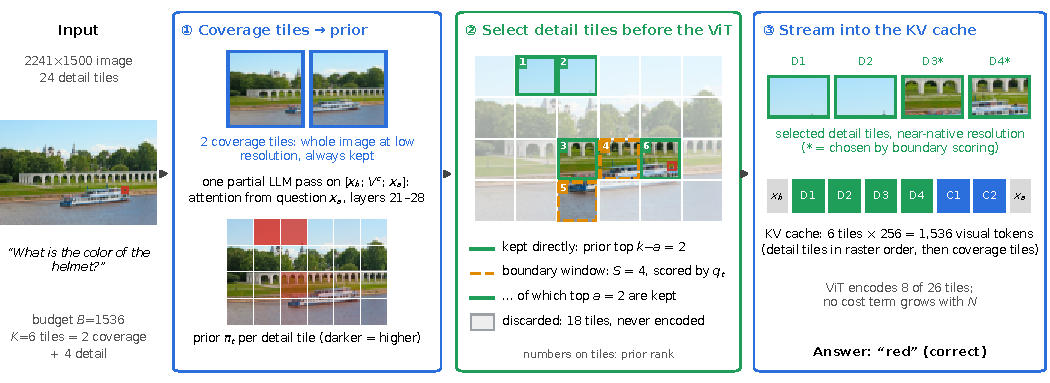
\includegraphics[width=\linewidth]{figures/fig_overview.pdf}
  \caption{\textbf{Overview of \method.} The image is represented at two scales: $m$ coverage tiles
  that show the whole image at low resolution, and a grid of $N$ detail tiles at near-native resolution.
  A single partial forward pass over the coverage tiles yields a question-aware prior over the detail
  tiles. The top-ranked tiles are kept directly, the tiles at the selection boundary are re-scored with
  question attention, and all other tiles are discarded \emph{before} the vision encoder. The selected
  tiles are streamed into the KV cache, so compute and memory are bounded by the budget $K$ rather than
  by $N$. Example from V$^*$~Bench~\cite{vstar} with $B=1536$ ($K=6$); the 3:2 image fits a $2\times1$ coverage grid, so the
  spare slot goes to the detail tiles. The prior ranks the target tile only sixth, and boundary scoring
  recovers it.}
  \label{fig:method}
\end{figure*}

% ─────────────────────────────────────────────────────────────────────────────
\subsection{Coverage tiles and detail tiles}
\label{sec:scales}

\method represents the image at two scales and splits the $K$ tile slots between them.

\paragraph{Coverage tiles.} The whole image is resized to a $c_c\times r_c$ grid of at most $m$ tiles,
where $m=\max(1,\lfloor K/2\rfloor)$. The official tiling optimizes only the aspect-ratio match and
often leaves part of such a budget unused. We instead pick the grid with the \emph{most} tiles,
$c_c r_c\le m$, among those whose aspect-ratio distortion is at most $1.75\times$, so that the coverage
tiles use their share of the budget. The coverage tiles are always kept. They give the model the global layout
and context of the image, and they are the input to the prior (\cref{sec:prior}).

\paragraph{Detail tiles.} The detail tiles are the official $c\times r$ grid with $N\le N_{\max}=47$
tiles, \ie close to native resolution. \method keeps $k=K-c_cr_c$ of them, so slots that the coverage grid
cannot fill go to detail tiles.

With $m=1$, the coverage tile reduces to the official thumbnail; the even split between the two scales
is calibrated (\cref{sec:impl}).

% ─────────────────────────────────────────────────────────────────────────────
\subsection{Question-aware prior from coverage tiles}
\label{sec:prior}

To rank the detail tiles without encoding them, we ask the VLM where it looks when it reads the question
against the low-resolution view. This builds on the observation that VLMs attend to the relevant region
even when they cannot resolve its details~\cite{vicrop}, which we quantified in \cref{sec:reliability}. We compute a single prior from the coverage
tiles, before any detail tile is encoded: we run the language
model on
$[\,\mathbf{x}_b;\ \mathbf{V}^{c};\ \mathbf{x}_a\,]$, where $\mathbf{V}^{c}\in\mathbb{R}^{nm\times d}$
are the coverage tokens, and stop after layer $l_{\text{hi}}$. Let $\mathbf{A}^{(l)}$ be the
head-averaged attention of layer $l$. The saliency of coverage patch $j$ is the attention it receives
from all text positions after the image, averaged over a band of middle-to-late layers
$\mathcal{L}_p=\{l_{\text{lo}},\dots,l_{\text{hi}}\}$, where visual information is transferred to the
question tokens~\cite{crossmodalflow}:
\begin{equation}
  s_j=\frac{1}{|\mathcal{L}_p|}\sum_{l\in\mathcal{L}_p}\frac{1}{|\mathbf{x}_a|}
      \sum_{i\in\mathbf{x}_a}\mathbf{A}^{(l)}_{i,j}.
  \label{eq:saliency}
\end{equation}
After min-max normalization, each coverage patch is assigned to the detail tile that contains its
center in normalized image coordinates, and the prior of detail tile $t$ is the mean saliency of its
patches, $\pi_t=\frac{1}{|P_t|}\sum_{j\in P_t}s_j$, again min-max normalized.

This pass costs a single forward over $|\mathbf{x}_b|+nm+|\mathbf{x}_a|$ tokens through
$l_{\text{hi}}$ of the $L$ layers, which is independent of $N$. We compute only the attention rows of
$\mathbf{x}_a$ in \cref{eq:saliency} and keep the fused attention kernel for the forward pass, so the
full attention matrix is never materialized. The pass also produces the KV cache of the prefix
$[\,\mathbf{x}_b;\ \mathbf{V}^{c}\,]$, which the next stage reuses.

% ─────────────────────────────────────────────────────────────────────────────
\subsection{Boundary scoring with question attention}
\label{sec:boundary}

The prior is computed at low resolution, so it can bring the target close to the top of the ranking but
cannot make the final choice on its own (\cref{sec:reliability}). \method therefore spends additional computation only on the tiles at the selection
boundary (\cref{fig:boundary}), similar to retrieve-then-rerank pipelines that apply an expensive scorer
only to the candidates of a cheap first stage~\cite{monobert}. Let the detail tiles be sorted by $\pi_t$, let $k$ be the number of
detail slots, and let $S$ be the size of the scoring window. With $a=\min(k,\lfloor S/2\rfloor)$, the top $k-a$ tiles are \emph{kept
directly} (encoded, not scored), the next $S$ tiles form the \emph{boundary window}, which is encoded and
scored and whose $a$ highest-scoring tiles are kept, and all remaining tiles are \emph{discarded} and never
reach the vision encoder.
The score of a boundary tile $t$ is its question attention at layer $l_q$, measured in the context of
the coverage tiles:
\begin{equation}
  q_t=\frac{1}{|\mathbf{x}_a|}\sum_{i\in\mathbf{x}_a}\ \sum_{j\in\mathbf{V}_t}
      \mathbf{A}^{(l_q)}_{i,j}
  \quad\text{on}\quad [\,\mathbf{x}_b;\ \mathbf{V}^{c};\ \mathbf{V}_t;\ \mathbf{x}_a\,].
  \label{eq:qattn}
\end{equation}
Because the prefix $[\,\mathbf{x}_b;\ \mathbf{V}^{c}\,]$ is shared by all candidates, its keys and values
for layers $1,\dots,l_q$ are taken from the prior pass, as in prompt caching~\cite{promptcache}. Each candidate therefore costs one pass of
$n+|\mathbf{x}_a|$ tokens through $l_q$ layers, and this is mathematically identical to a full forward
over the sequence in \cref{eq:qattn}. Since $q_t$ depends only on tile $t$ and the question, the top-$a$
selection can be made on the fly with a size-$a$ min-heap while the window is streamed, without holding
all candidates in memory. Setting $S=0$ reduces \method to prior-only selection.


% ─────────────────────────────────────────────────────────────────────────────
\subsection{Streaming KV construction}
\label{sec:streaming}

\method builds the KV cache incrementally. It first prefills $\mathbf{x}_b$, then encodes the coverage
tiles and runs the prior. The candidate detail tiles, \ie the directly kept tiles and the boundary window,
are encoded in raster order in micro-batches of four tiles; boundary tiles are scored as they arrive and
enter or leave the size-$a$ pool. Once selection is final, the selected detail tiles are written to the
KV cache in raster order, followed by the $m$ coverage tiles. This mirrors the order seen in training,
where grid tiles precede the global thumbnail. The visual tokens are prefilled in chunks of 1{,}024
tokens with contiguous position ids after $\mathbf{x}_b$. Finally, $\mathbf{x}_a$ is prefilled and the
answer is decoded from the resulting cache of at most $|\mathbf{x}_b|+nK+|\mathbf{x}_a|$ tokens. The
visual tokens resident in memory never exceed about $k+m$ tiles plus one micro-batch, \ie
$\mathcal{O}(K)$.


\paragraph{Cost.}
\cref{tab:complexity} summarizes the cost per image. \method encodes $c_cr_c+(k-a)+S=K-a+S$ tiles. Its
language-model work consists of the prior pass over $|\mathbf{x}_b|+nm+|\mathbf{x}_a|$ tokens
($l_{\text{hi}}$ layers), $S$ scoring passes of $n+|\mathbf{x}_a|$ tokens ($l_q$ layers), and the main
prefill of $nK$ visual tokens. Every term depends on the budget $K$ and the window $S$, but none depends
on the number of tiles $N$ (per-stage timings in \cref{tab:ttft}). The KV cache is bounded by the budget. In contrast, every method that prunes
after encoding pays $\mathcal{O}(N)$ vision compute, and methods that prune inside the language model
also pay $\mathcal{O}(N)$ in the layers before pruning.

\begin{table}[t]
  \centering
  \small
  \setlength{\tabcolsep}{4pt}
  \begin{tabular}{lccc}
    \toprule
    Method & ViT & LLM prefill & KV cache \\
    \midrule
    Uncompressed & $N$ & $N$ & $N$ \\
    VisionZip, HiRED & $N$ & $K$ & $K$ \\
    FastV, SparseVLM & $N$ & $N\!\to\!K$ & $\approx K$ \\
    IF-Prune & $N^{\ddagger}$ & $N\!\to\!K$ & $\approx K$ \\
    \method (ours) & $K{-}a{+}S$ & $K{+}m{+}S^{\dagger}$ & $K$ \\
    \bottomrule
  \end{tabular}
  \caption{\textbf{Cost per image} in units of tiles ($n=256$ tokens each), with $N$ detail tiles and a
  budget of $K$ tiles; text tokens are omitted. $N\!\to\!K$: all $N$ tiles pass through the layers
  before pruning, $K$ remain after. $^{\ddagger}$Plus a 1B guide VLM on all $N$ tiles.
  $^{\dagger}$The $m$ coverage and $S$ boundary tiles pass only through the first $l_{\text{hi}}$ and
  $l_q$ layers. Only \method is independent of $N$.}
  \label{tab:complexity}
\end{table}

% ─────────────────────────────────────────────────────────────────────────────
\subsection{Hyperparameters and calibration}
\label{sec:impl}

\method has no trained parameters. The coverage fraction $m/K$, the window $S$ for each budget, and the default
budget are set once on held-out data and frozen for all test sets: 600 questions from the InfoVQA \emph{train}
split and 600 from MME-RealWorld outside its Lite subset and images, which share no questions or images with any
test set. On these sets, $m/K=0.5$ is within 0.1 points of the best average accuracy and has the most stable
worst-task accuracy, whereas the thumbnail alone ($m=1$) is about 7 points lower (\cref{tab:ablation}). Without
boundary scoring ($S=0$), remote sensing questions lose up to 10.8 raw points, while windows up to four times
larger give no reliable gain, so we use $S=\{5,4,4,3,3\}$ for $B=\{1024,1536,2048,2560,3072\}$. The default
$B=1536$ ($K=6$, $m=3$, $S=4$) is where held-out accuracy saturates. The attention layers,
$\mathcal{L}_p=\{21,\dots,28\}$ and $l_q=20$ for InternVL3.5-8B ($L=36$), were fixed in preliminary experiments
before this protocol. The full protocol, including deviations from our pre-registered rules, is in the
supplementary material.

% NOTE: L_p and l_q were chosen on InfoVQA val before the held-out protocol existed
% (docs/04_calibration_protocol.md, 1.8.3 note). Disclose this in the supplementary.
